\documentclass[a4paper,14pt]{article} % тип документа
%\documentclass[14pt]{extreport}
\usepackage{extsizes} % Возможность сделать 14-й шрифт


\usepackage{geometry} % Простой способ задавать поля
\geometry{top=25mm}
\geometry{bottom=35mm}
\geometry{left=20mm}
\geometry{right=20mm}

\setcounter{section}{0}

%%%Библиотеки
%\usepackage[warn]{mathtext}
%\usepackage[T2A]{fontenc} % кодировка
\usepackage[utf8]{inputenc} % кодировка исходного текста
\usepackage[english,russian]{babel} % локализация и переносы
\usepackage{caption}
\usepackage{listings}
\usepackage{amsmath,amsfonts,amssymb,amsthm,mathtools}
\usepackage{wasysym}
\usepackage{graphicx}%Вставка картинок правильная
\usepackage{float}%"Плавающие" картинки
\usepackage{wrapfig}%Обтекание фигур (таблиц, картинок и прочего)
\usepackage{fancyhdr} %загрузим пакет
\usepackage{lscape}
\usepackage{xcolor}
\usepackage{dsfont}
%\usepackage{indentfirst}
\usepackage[normalem]{ulem}
\usepackage{hyperref}




%%% DRAGON STUFF
\usepackage{scalerel}
\usepackage{mathtools}

\DeclareMathOperator*{\myint}{\ThisStyle{\rotatebox{25}{$\SavedStyle\!\int\!\!\!$}}}

\DeclareMathOperator*{\myoint}{\ThisStyle{\rotatebox{25}{$\SavedStyle\!\oint\!\!\!$}}}

\usepackage{scalerel}
\usepackage{graphicx}
%%% END 

%%%Конец библиотек

%%%Настройка ссылок
\hypersetup
{
colorlinks=true,
linkcolor=blue,
filecolor=magenta,
urlcolor=blue
}
%%%Конец настройки ссылок






\begin{document}
%%%%Начало документа%%%%
Решается задача регрессии.
На подвыборках, равномощных выборке, оцениваются параметры. По K подвыборкам получены матожидание и дисперсия 
каждого параметра модели. Требуется построить график ($\lambda, \omega_j$), где $\lambda $ -- коэффициент регуляризации
функции ошибки.	


1) $S = ||f-y||_2^2 + \lambda_2||w||_2^2$

2) $S = ||f-y||_2^2 + \lambda_1||w||_1$

3) $S = ||f-y||_2^2 + \lambda_2||w||_2^2 + \lambda||w||_1$

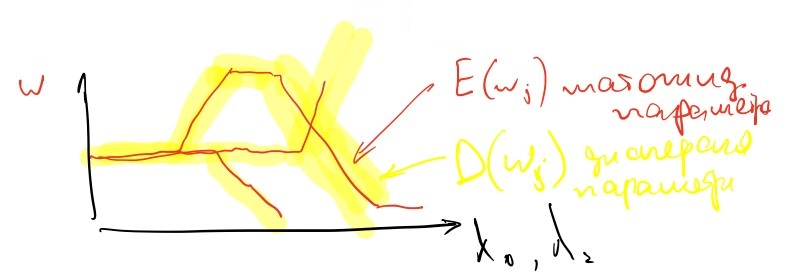
\includegraphics[scale=0.78]{00.jpg}


Пусть $F = f(\omega, X) = X_{m \cdot n} w_{n \cdot 1}$ - модель

$(X, y_{m \cdot 1})$ - выборка

%Быстрый вопрос: понятна ли задача?
\newpage
\section{Решение:}
\subsection{I}
\begin{equation}
S = ||Xw - Y||_2^2 + \lambda_2||w||_2^2
\end{equation}

\begin{equation}
S = (Xw - Y)^T(Xw-Y) + \lambda_2w^Yw = Y^TY - 2Y^TXw + w^TX^TXw + \lambda_2w^Tw
\end{equation}

\begin{equation}
grad_wS = -2X^TY+2X^TX\omega+2\lambda_2\omega = 0
\end{equation}

\begin{equation}
\omega = (X^TX + \lambda_2E)^{-1}X^TY
\end{equation}

Я пробовал преобразовать систему и попытаться решить, её но это сводится к поиску обратной матрицы.
И пришел к тому, что нужно попытаться представить как-то матрицу X.
Воспользуемся сингулярным разложением: $X = V D U^T$, где D -- диагональная матрица из корней собственных значений матриц $X^TX$ и $XX^T$, U, V -- эрмитовы (U составлена из собственных векторов матрицы $X^TX$, V составлена из собственных векторов матрицы $XX^T$)

Тогда получим:
\begin{equation}
    \omega = (U D V^T V D^T U^T + \lambda_2 E)^{-1}UD^TV^TY
\end{equation}
\begin{equation}
    \omega = (U DD^T U^T + U \lambda_2 EU^T)^{-1}UD^TV^TY
\end{equation}

\begin{equation}
    \omega = (U^T)^{-1}(D^2 + \lambda_2 E)^{-1}UUDV^TY
\end{equation}

\begin{equation}
    \omega = U(D^2 + \lambda_2 E)^{-1}DV^TY
\end{equation}

\begin{equation}
    \omega = \sum\limits_{i = 1}^n\frac{\sqrt{\lambda_i}}{\lambda_i + \lambda_2}u_i(v_jY)
\end{equation}

Т.е. получили, что $w_j(\lambda_2) = \sum\limits_{i = 1}^n \frac{c_{1, i}}{\lambda_i + \lambda_2}$, где $c_{1, i}$ -- какая-то константа полученная от перемножения матриц и соотвествующего коэффициента в $u_i$ и корня из собственного числа.

\subsection{II}
Теперь рассмотрим для: $S = ||X\omega - Y||_2^2 + \lambda_1||\omega||_1$
\begin{equation}
    S = (X\omega - Y)^T(X\omega - Y) + \lambda_1||\omega||_1
\end{equation}

\begin{equation}
    S = Y^TY - 2Y^TX\omega + \omega^TX^TX\omega + \lambda_1 \sum\limits_{i = 1}^n |w_i|
\end{equation}

%Теперь заменим, $\omega_i = \omega_i^+ - \omega_i^-$ и получим, что $|\omega_i| = \omega_i^+ + \omega_i^-$ 

\begin{equation}
    grad_wS = -2X^TY+2X^TX\omega + 2\lambda_1 sign(\omega)   = 0
\end{equation}


\begin{equation}
    \omega = (X^TX)^{-1}(X^TY - \frac{\lambda_1}{2} sign(\omega))
\end{equation}

\begin{equation}
    \omega = (UD^TV^TVDU^T)^{-1}(UD^TV^T - \frac{\lambda_1}{2}sign(\omega))
\end{equation}

\begin{equation}
    \omega = (UD^TV^TVDU^T)^{-1}(UD^TV^T - \frac{\lambda_1}{2}sign(\omega))
\end{equation}

\begin{equation}
    \omega = \sum\limits_{i = 1}^n (\frac{u_i}{\sqrt{\lambda_i}}(v_i, Y) - \frac{\lambda_1}{2 * \lambda_i}u_i(u_i^T, sign(\omega)))
\end{equation}

\subsection{III}
\begin{center}
Для случая $S = ||X\omega - Y||_2^2 + \lambda_2||\omega||_2^2 + \lambda_1||\omega||_1$


\begin{equation}
    grad_wS = -2X^TY+2X^TX\omega+2\lambda_2\omega + \lambda_1 sign(\omega) = 0
\end{equation}

\begin{equation}
    \omega = (X^TX + \lambda_2E)^{-1}(X^TY - \frac{\lambda_1}{2}sign(\omega))
\end{equation}

\begin{equation}
    \omega = \sum\limits_{i = 1}^n \frac{\sqrt{\lambda_i}}{\lambda_i + \lambda_2}\left( u_i(v_j, Y) - \frac{\lambda_1}{2}(u_i, u_i^T)sign(\omega)\right)
\end{equation}

\begin{equation}
    \omega_j = \sum\limits_{i = 1}^n \frac{\sqrt{\lambda_i}}{\lambda_i + \lambda_2} (u_{i, j}(v_i, Y) - \frac{\lambda_1}{2}u_{i, j}(u_i^T, sign(\omega)))
\end{equation}

\end{document} 